\section{Overview} %TODO Maybe remove this
\textbf{Magnetic Resonance Imaging} (\textbf{MRI}) is an imaging modality that expoits the phenomenon of Nuclear Magnetic Resonance to record information about the local chemical environment of specific atoms within a body. Commonly, these atoms are the hydrogen nuclei, but MRI is possible with any nuclei with a non-integer nuclear spin. Generally, the proceedure for MRI is summarized in the following steps, where only step \ref{item:mri:gensteps:gradients} is specific to the Imaging modality over an NMR experiment:
\begin{enumerate}
	\item \label{item:mri:gensteps:b0} Nuclei align with an applied, strong magnetic field $\vec{B}_0$.
	\item \label{item:mri:gensteps:rf} Radio Frequency energy is applied to flip the nuclear magnetization off-axis from $\vec{B}_0$.
	\item \label{item:mri:gensteps:precess} Interaction between $\vec{B}_0$ and nuclear magnetizations causes magnetizations to \textbf{\textit{precess}}.
	\item \label{item:mri:gensteps:record} Induced current from precessing magnetization is observed in an RF coil.
	\item \label{item:mri:gensteps:gradients} Speed of precession is spatially varied by a spatially-varying magnetic field gradient.
\end{enumerate}
\section{Magnetism and Nuclear Magnetic Resonance}
Magnetism is an inherent property of matter which causes materials to interact with external magnetic fields to generate their own magnetic field. This phenomenon is characterized by the relation
\begin{equation}
\vec{H} = \chi \vec{B} \label{eq:mri:magneticsusceptibility}
\end{equation}
where $\vec{H}$ is the generated field, $\vec{B}$ is the applied field, and $\chi$ is the \textit{magnetic susceptibility} of the matter. Matter is classified into three main categories based on $\chi$:
\begin{description}
	\item[Paramagnetic] matter has \textit{positive} $\chi$, thus $\vec{H}$ points in the same direction as $\vec{B}$. \textbf{Ex:} Aluminum
	\item[Diamagnetic] matter has \textit{negative} $\chi$, thus $\vec{H}$ points in the opposite direction as $\vec{B}$. \textbf{Ex:} Water
	\item[Ferromagnetic] matter has \textit{large} $\chi$. \textbf{Ex:} Iron
\end{description}
Magnetism originates from the electrons of an atom, but Nuclear Magnetic Resonance originates from the nucleus and is still subject to electronic magnetism, or \textit{chemical shift} phenomena.

Nuclear Magnetism arises from nuclei of atoms with odd-even pairing of neutrons and protons, resulting in nuclei with non-integer spin. E.g. $^1$H with spin $I=\sfrac{1}{2}$. Nuclear spin in motion gives rise to an angular momentum of the spin:
\begin{equation}
J=\hbar I = \frac{h}{2\pi}I
\end{equation}
where J is the resulting angular momenta, $h$ is Planck's constant, and $\hbar$ is the reduced Planck constant. 
The magnetic moment of matter is also determined by
\begin{equation}
\mu = \gamma J = \gamma \hbar I
\end{equation}
where $\mu$ is the magnetic moment and $\gamma$ is the \textit{gyromagnetic ratio} that is specific to the nucleus in question.

Bulk magnetization (the collective net magnetization from a region of matter) is dependent upon the relative number of individual moments in the `up' (parallel to $\vec{B}_0$) and `down' (anti-parallel to $\vec{B}_0$) states:
\begin{equation}
\vec{m} = \mu (\Delta N)
\end{equation}
where $N$ is the number of magnetic moments in the up and down states such that $\Delta N$ is the net difference of moments in the anti-parallel direction.
$N$ follows a Boltzmann distribution based on the energy state, $E$, of the nuclei:
\begin{equation}
N\propto e^{-\frac{E}{kT}}
\end{equation}
where $k$ is the Boltzman constant and $T$ is the absolute temperature. The energy state of a magnetic moment is
\begin{equation}
E(\mu) = -\mu B_0 = -\gamma \hbar m B_0
\end{equation}
where $m = \left\{I \ldots\sfrac{3}{2}, \sfrac{1}{2}, -\sfrac{1}{2}, -\sfrac{3}{2},\ldots -I\right\}$ are the permissible states for the spin $I$. Again assuming $^1$H nuclei, the two energy states are
\begin{align}
E\left(\text{up}\right) &= - \gamma \hbar \left(\sfrac{1}{2}\right) B_0 \\
E\left(\text{down}\right) &= + \gamma \hbar \left(\sfrac{1}{2}\right) B_0 .
\end{align}
The ratio of spin alignment can then be calculated:
\begin{equation}
\frac{N\left(\text{up}\right)}{N\left(\text{down}\right)} = e^{+ \frac{\Delta E}{kT}} \label{eq:mri:ratio}
\end{equation}
where $\Delta E = E\left(\text{down}\right) - E\left(\text{up}\right)$. If we then suppose that there exist a total of $N$ nuclei such that $N\left(\text{up}\right) + N\left(\text{down}\right) = N$, then from this and (\ref{eq:mri:ratio}) we can solve for $\Delta N$ and thus $M$:
\begin{equation}
M=\mu \Delta N = \frac{N\gamma^2 \hbar^2 B_0}{4kT}
\end{equation}
This equation can be massaged to match the form of (\ref{eq:mri:magneticsusceptibility}):
\begin{align}
M = \chi_{_0} B_0 && \chi_{_0} = \frac{N\gamma^2 \hbar^2 }{4kT}
\end{align}
where $\chi_{_0}$ is a matter-specific term that describes the resulting magnetic field from an applied field $B_0$. This $\chi_{_0}$ is very small, and results in a very low effective signal from a body of matter. However, there are engineering decisions in each of these terms that helps raise the signal:
\begin{description}
	\item[$\mathbf{B_0}$] Make it big, but not too big. Like 1.5 T at least, probably 7 T is awesome.
	\item[$\mathbf{N}$] Effectively this is the voxel size. Cubic power. $\sfrac{1}{2}$ resolution $\to$ 8x larger voxel $\to$ 64x signal.
	\item[$\mathbf{T}$] Very limited range if you want the subject to be alive, but colder is better.
	\item{$\!\!\mathbf{\gamma}\;$} Pick nuclei with high $\gamma$, and isotope with high abundance. See Table \ref{tab:mri:nuclist}.
\end{description}
\begin{table}[h]
	\caption{\label{tab:mri:nuclist} Relevant Properties of Some Common Nuclei}
	\centering
	\begin{tabular}{|c|c|c|c|}
		\hline Nuclei & $I$ & $\frac{\gamma}{2\pi}$ (MHz/T) & nat. abundance (\%) \\ 
		\hline $^1$H & \sfrac{1}{2} & \textbf{42.58} & 99.98 \\ 
		\hline $^{13}$C & \sfrac{1}{2} & 10.71 & 1.11 \\ 
		\hline $^{19}$F & \sfrac{1}{2} & 40.05 & 100 \\ 
		\hline $^{31}$P & \sfrac{1}{2} & 17.23 & 100 \\ 
		\hline $^{23}$Na & \sfrac{3}{2} & 11.26 & 100 \\ 
		\hline 
	\end{tabular} 
\end{table}

\section{Spin Motion and the NMR Signal}
Precession of the nuclear magnetization, or `spin' is described by
\begin{equation}
\frac{d\vec{m}}{dt}=\gamma \vec{m} \times \vec{B}.
\end{equation}
The resulting motion is analogous to a spinning gyroscope: the rotation does not change, but the \textit{axis of rotation} changes. The precession of earth leads to changes in the classification of the north star, while the typical spinning of earth manifests as day/night.

There are four important cases of spin motion in the context of MRI/NMR:
\begin{enumerate}
	\item First is the case when $\vec{m}$ is aligned with $\vec{B}$, for example $\vec{m} = m_0\; \hat{z}$ and $\vec{B}  = B_0\; \hat{z}$. This results in the derivative term being zero from properties of the vector cross product. This case is stable (see Fig. \ref{fig:mri:stable}).

\item \label{item:mri:precession}The second case is substantially more interesting. If we let 
\begin{equation}
\vec{m} = m_0\; \hat{x}
\end{equation} and \begin{equation}
\vec{B}  = B_0\; \hat{z} ,
\end{equation} then \begin{equation}
 \frac{d\vec{m}}{dt} = - m_0B_0\;\hat{y}\; .
 \end{equation} 
This results in the infinitesimal motion of the magnetization to move in the $-\hat{y}$ direction. As time progresses, the magnetization precesses \textit{about} $-\hat{z}$ at the rate $\omega = -\gamma B_0$, known as the \textit{Larmor} frequency (see Fig. \ref{fig:mri:precession}).
\item Similar to case \ref{item:mri:precession}, the precession about $-\hat{z}$ is stable at any angle $\alpha$ (see Fig. \ref{fig:mri:decay}).

\item Finally, the case of `flipping' the magnetization from alignment with $\hat{z}$ to alignment with $\hat{x}$. Starting with \begin{equation}
\vec{m} = m_0\; \hat{z}
\end{equation} the application of an infinitely short magnetic field pointing in the $-\hat{y}$ direction 
\begin{equation}
\vec{B} = -\delta(t)B_1\hat{y}
\end{equation}results in changing the direction of $\vec{m}$ towards the $\hat{x}$ axis. Realistically, this applied field cannot be infinitely short, so after every bit of time, the $\vec{B}_1$ field must be updated to still be perpendicular to $\vec{m}$. This results in a field applied according to
\begin{equation}
\vec{B}=B_1\big(\cos\left(\omega_0 t\right) - \sin\left(\omega_0 t\right)\big)
\end{equation}
giving a clockwise spin of the applied magnetic field (precession about the $-\hat{z}$ axis). This results in $\vec{m}$ precessing about the $\hat{z}$ axis while being progressively `flipped' to the transverse ($\hat{x}$-$\hat{y}$) plane. The overall `flip' procedure is parameterized by $\alpha$, the resulting angle that $\vec{m}$ makes with the $+\hat{z}$ axis (see Fig. \ref{fig:mri:flip}).

\end{enumerate}

\begin{figure}[h]
	\centering
	\begin{subfigure}[b]{0.22\textwidth}
		\centering
		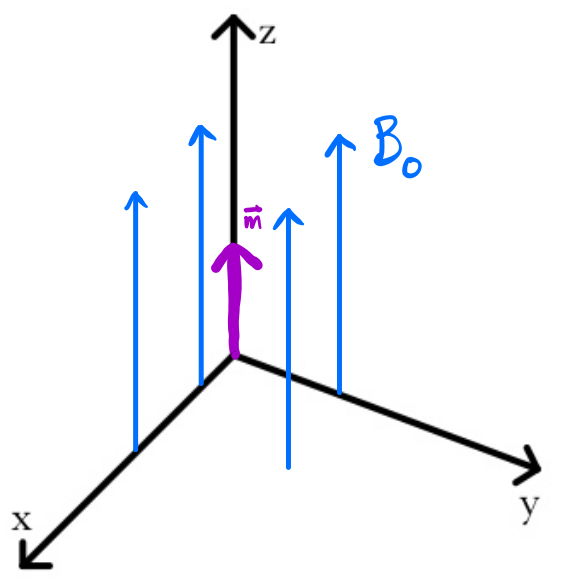
\includegraphics[width=\linewidth]{mri-a}
		\caption{Stable Magnetization}
		\label{fig:mri:stable}
	\end{subfigure}\hfill
	\begin{subfigure}[b]{0.22\textwidth}
		\centering
		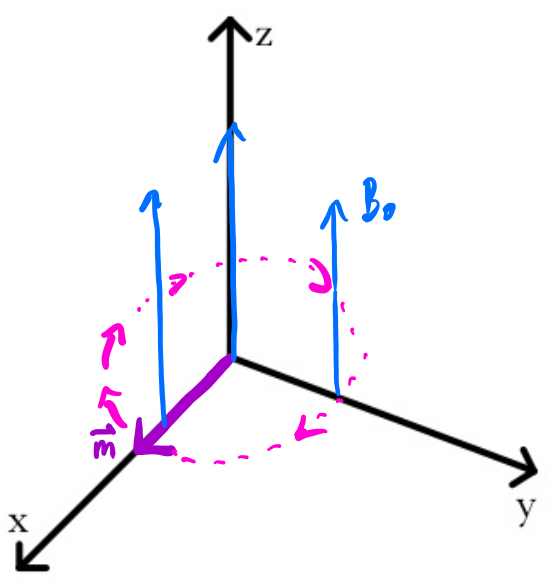
\includegraphics[width=\linewidth]{mri-b}
		\caption{Spin Motion}
		\label{fig:mri:precession}
	\end{subfigure}\hfill
	\begin{subfigure}[b]{0.22\textwidth}
		\centering
		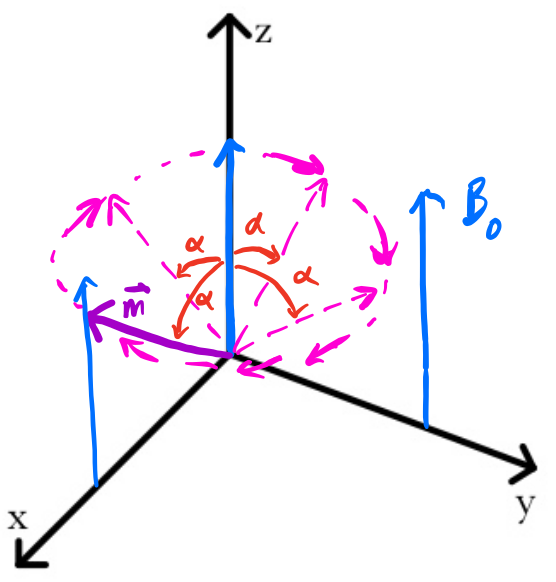
\includegraphics[width=\linewidth]{mri-c}
		\caption{Precession at an angle}
		\label{fig:mri:decay}
	\end{subfigure}\hfill
	\begin{subfigure}[b]{0.22\textwidth}
		\centering
		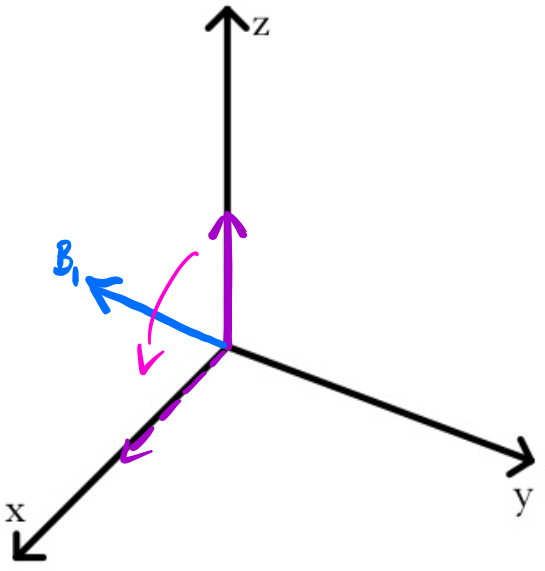
\includegraphics[width=\linewidth]{mri-d}
		\caption{Excitation}
		\label{fig:mri:flip}
	\end{subfigure}
	\caption{Canonical Cases of Spin Motion}\label{fig:mri:cases}
\end{figure}

The fundamentals presented thus far are sufficient to describe the most basic NMR experiment:\\
{\centering
	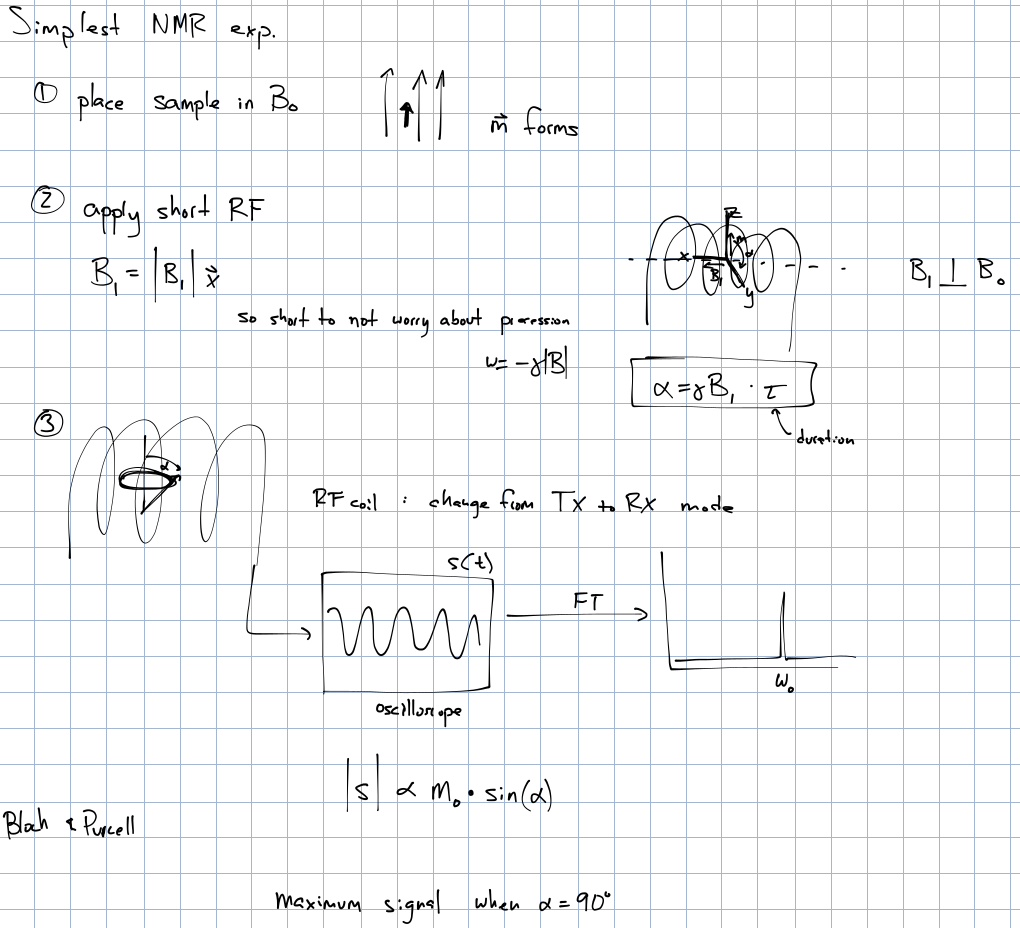
\includegraphics[width=0.8\linewidth]{mri-nmr}
}

\section{Spatial Encoding}
Magnetic Resonance \textit{Imaging} is made possible by encoding spatial information in the NMR signal. This is accomplished by making $B$ a linear function of space using \textit{gradient fields}. These magnetic gradient fields are always parallel to the main $B_0$ field. By changing the magnitude of the magnetic field, the spins precess faster or slower to form a frequency histogram, which is a projection of the object. Example gradient fields are shown in Fig. \ref{fig:mri:gradients}.

\begin{figure}[h]
	\centering
	\begin{subfigure}[b]{0.3\textwidth}
		\centering
		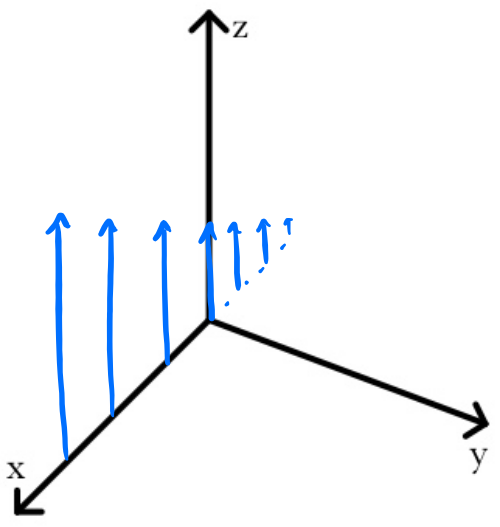
\includegraphics[width=\linewidth]{mri-gradx}
		\caption{$G_x$}
		\label{fig:mri:gradx}
	\end{subfigure}\hfill
	\begin{subfigure}[b]{0.3\textwidth}
		\centering
		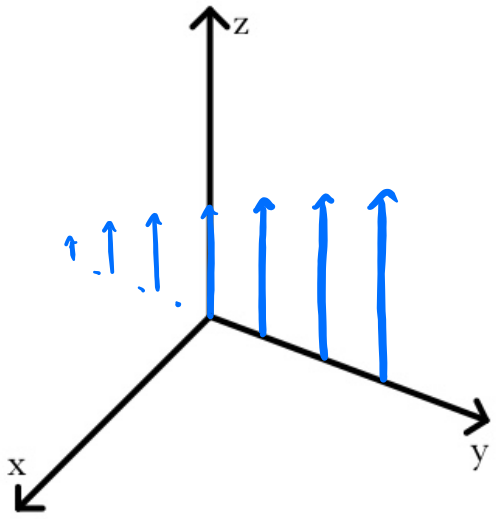
\includegraphics[width=\linewidth]{mri-grady}
		\caption{$G_y$}
		\label{fig:mri:grady}
	\end{subfigure}\hfill
	\begin{subfigure}[b]{0.3\textwidth}
		\centering
		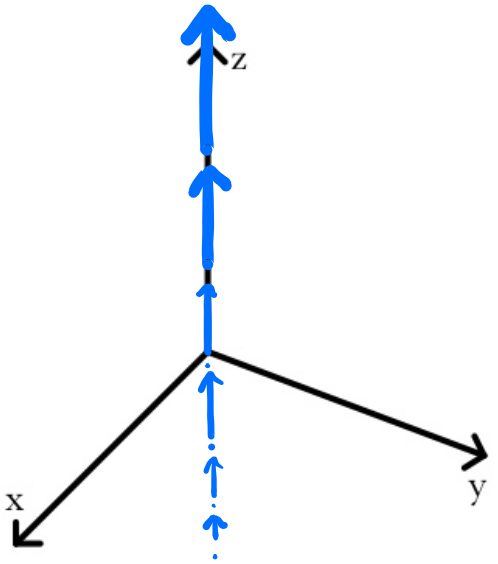
\includegraphics[width=\linewidth]{mri-gradz}
		\caption{$G_z$}
		\label{fig:mri:gradz}
	\end{subfigure}
	\caption{Gradient Fields}\label{fig:mri:gradients}
\end{figure} 

The Larmor frequency is thus dependent on the location of the spin:
\begin{align}
\vec{G} &= \left[\begin{matrix}G_x\\G_y\\G_z\end{matrix}\right]\\
\vec{r} &= \left[\begin{matrix}x\\y\\z\end{matrix}\right]\\
B &= B_0 + \vec{G}\cdot \vec{r}\\
\omega(\vec{r}) &= -\gamma B = -\gamma\left(B_0 + \vec{G}\cdot \vec{r}\right) \label{eq:mri:larmorgrad}
\end{align}
Using this relation and assuming that $m(x,y,z) = m(\vec{r})$ is the proton density image, each magnetization in space will precess at the frequency corresponding to its location by \ref{eq:mri:larmorgrad}. The signal radiated by a single point is 
\begin{equation}
m(\vec{r})e^{i\omega(\vec{r})t}.
\end{equation}
The total signal recorded by a coil surrounding the body is found by integrating over the entire volume:
\begin{equation}
s(t) = \iiint_{\Omega}m(\vec{r})e^{-i\gamma \vec{G}\cdot\vec{r}t}d\vec{r}
\end{equation}
A useful substitution is made by introducing the variable $k$:
\begin{equation}
\vec{k} = \frac{\gamma}{2\pi} \vec{G}t
\end{equation}
\begin{equation}
s(\vec{k}) = \iiint_{\Omega}m(\vec{r})e^{-i2\pi \vec{k}\cdot\vec{r}}d\vec{r}
\end{equation}

Close inspection of this equation reveals that it is simply the forward Fourier Transform of the function of spatial magnetization $m(\vec{r})$. The original magnetization image can be easily obtained by the \textit{inverse} Fourier Transform of the acquired signal.
\section{Slice Selection}
Spatial encoding of the Larmor frequency via gradient fields also enables selective excitation. The target nuclei within the 2D plane (or slab) we aim to excite are provisioned a common resonant frequency by applying a gradient in the direction orthogonal to that plane. The target slice can then be excited by delivering radiofrequency energy at the appropriate frequency via a modulated radiofrequency pulse, especially a sinc-modulated sinusoid. 


\section{MRI Contrast Mechanisms}
\subsection{Spin Lattice Relaxation - T1}
\begin{equation}
\frac{dm_z}{dt}= \frac{m_0-m_z}{T_1}
\end{equation}

\begin{equation}
m_z(t) = \underset{\text{initial condition}}{\underbrace{\qquad\qquad}} e^{\frac{-t}{T_1}} + \underset{\text{final condition}}{\underbrace{\quad m_0\quad}}\left(1-e^{\frac{-t}{T_1}}\right)
\end{equation}

add graph here


\subsection{Spin-Spin Relaxation - T2}
\begin{equation}
T_2 << T_1
\end{equation}

\begin{equation}
\frac{dm_{xy}}{dt}= \frac{-1}{T_1}m_{xy}
\end{equation}

\begin{equation}
m_{xy}(t) = \underset{\text{initial condition}}{\underbrace{\qquad\qquad}} e^{\frac{-t}{T_2}}
\end{equation}

add graph here

\subsection{Dephasing - T2*}
Same as $T_2$, just faster, due to $B_0$ inhomogeneity, spins dephase in $xy$ plane.
\subsection{Bloch Equation}
The $T_1$ and $T_2$ contrast mechanisms are incorporated together in the spin motion equation to fully describe the motion of a nuclear spin through time. In pieces, the equations are the same as what was introduced above in each section.
\begin{align}
\frac{d\vec{m}}{dt} &= \gamma \vec{m} \times \vec{B}  \\
\frac{dm_z}{dt}&= \frac{m_0-m_z}{T_1} =\frac{m_z-m_0}{T_1} \\
\frac{dm_{x}}{dt}&= \frac{-m_{x}}{T_1}  \\
\frac{dm_{y}}{dt}&= \frac{-m_{y}}{T_1}
\end{align}
These equations are written together as a single vector equation:
\begin{equation}
\frac{d\vec{m}}{dt} = \gamma \vec{m} \times \vec{B} -\left[\begin{matrix}\sfrac{1}{T_2}&0&0\\0&\sfrac{1}{T_2}&0\\0&0&\sfrac{1}{T_1}\end{matrix}\right] \left(\vec{m}-\vec{m}_0\right)
\end{equation}
\subsection{Diffusion}
\subsection{FatSat}